% This is a latex file for Journal Club report 


% Author: Viswambhar Yasa
\documentclass[a4paper,12pt,times]{article}

% This are some packages used in bulding the report 
\usepackage{amsmath} 
\usepackage{graphicx}
\usepackage{multirow}
\usepackage{fancyvrb,color}
\usepackage{float}
\usepackage{amsmath}
\usepackage{geometry}
\usepackage[sort&compress,square,comma,numbers]{natbib}
\usepackage{wrapfig, blindtext}
\usepackage{index}
\usepackage[intoc]{nomencl}
\usepackage{subfig}
\usepackage{matlab-prettifier}
\usepackage{csvsimple}
\usepackage[english]{babel}
\usepackage{hyperref}
\hypersetup{
    colorlinks=true,
    linkcolor=blue,
    filecolor=blue,      
    urlcolor=blue,
}
\usepackage{listings}
\usepackage{color}

\definecolor{dkgreen}{rgb}{0,0.6,0}
\definecolor{gray}{rgb}{0.5,0.5,0.5}
\definecolor{mauve}{rgb}{0.58,0,0.82}

\lstset{frame=tb,
  language=Python,
  aboveskip=3mm,
  belowskip=3mm,
  showstringspaces=false,
  columns=flexible,
  basicstyle={\small\ttfamily},
  numbers=none,
  numberstyle=\tiny\color{gray},
  keywordstyle=\color{blue},
  commentstyle=\color{dkgreen},
  stringstyle=\color{mauve},
  breaklines=true,
  breakatwhitespace=true,
  tabsize=3
}


\setlength{\parindent}{1em}
\setlength{\parskip}{0.5em}
\renewcommand{\baselinestretch}{1}

\def\myauthor{Viswambhar Reddy Yasa} % Author
\def\matriculationno{65074} 
\def\mytitle{iso-geometric analysis based topology optimization (igto) }
\def\mydate{\today} 

%start  of the main documnt
\begin{document}

\begin{center}
    \textsc{Personal Programming Project 2020-21 }\\
    \vspace*{0.5 cm}
    {\LARGE \textsc{\mytitle}} %Title 
    \vspace{0.025\textheight}
    \rule{0.75\textwidth}{0.45pt}\\
    {\large \textsc{\myauthor}}\\ % Name
    \vspace{0.025\textheight}
    {\textsc{Computational Material Science}}\\
	\vspace{0.025\textheight}
	{65074}\\
\end{center}
\begin{section}{User manual}
The following steps should be performed to run the program and test cases. All the files are written in python.
\begin{figure}[H]
	\begin{center}
		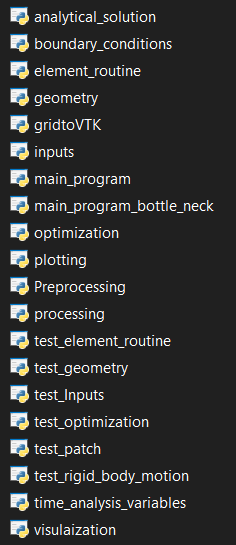
\includegraphics[scale=0.75]{list_of_files.png} 
		\caption{List of all python files}\label{list of files}
	\end{center}	
\end{figure}
\begin{subsection}{Procedure to run the program}
All python files have to be placed in same folder and working directory has to be same to run the python program. Any python environment can be used to run this python code.

\begin{enumerate}
    \item A file name main$\_$program.py is the starting point of the IGTO program.\\
    command: \textbf{python main$\_$program.py} 
    \begin{enumerate}
        \item Required python external libraries like 'numpy', 'matplotlib', 'pyvista', 'pyEVTK','pytest' are checked and installed.
       \begin{figure}[H]
	\begin{center}
		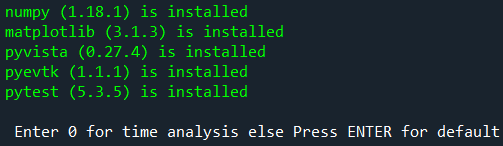
\includegraphics[scale=1]{installed_lib.png} 
		\caption{Installed python libraries}\label{installed python}
	\end{center}	
\end{figure}
    \end{enumerate}
    \item A prompt appears which asks the user to choose if time analysis has to be performed or not.\\ 
    0- Time analysis (log files are generated)\\
    Enter - For normal execution without any log files.
    
    \item Then the inputs have to be given or press enter to run default values.
    \begin{lstlisting}
l h w nx ny nz load volume_fra penal rmin E v density BC_op Ft_op verbose
8 5 1 35 25 3 -100 0.4 3 1.5 150000 0.3 7850 0 1 1
INPUTS WITH DEFAULT VALUES:
Length(l)							: 8     
Height(h)							: 5
Width(w)								: 1
nx(no of elements along x)	: 35
ny(no of elements along y)  : 25
nz(no of elements along z)	: 3
load									: -100
volume_fraction					: 0.4
penal									: 3
rmin									: 1.5
E(Youngs modulus)					: 150000
v(poisson ratio)					: 0.3
density								: 7850
BC_op									: 0
Ft_op									: 1
verbose								: 1

    \end{lstlisting}
    
Boundary condition option (BC$\_$op):\\
    \begin{lstlisting}

Option :
0- Cantilever beam with load along the bottom edge of the free end.
1- Simple supported with point load at bottom center.
2- Cantilever beam with point load at bottom of the free end.
3- Cantilever beam with point load at the free end (2d case loading at y=height and x=length).
4- Cantilever beam with two forces at top and bottom of the free end .
5- Cantilever beam with point load at the center of the free end.
6- Simple supported with load at top center.
    \end{lstlisting}
Optimizer option (Ft$\_$op):\\
    \begin{lstlisting}
Option :
0-OC (optimality criterion)

1-MMA (method of moving asymptotes)
    \end{lstlisting}
 Verbose:\\
     \begin{lstlisting}
Option :
0-Will not print plots using pyvista only VTK file is generated.

1- Plots are generated and stored in results folder.
    \end{lstlisting}
\item Plots are stored in respective sub folder with optimizer names in results folder.

\item A copy of input values and time log file are stored in log$\_$files folder.
\end{enumerate}
\end{subsection}
\begin{subsection}{Procedure to run the test case}
We used pytest to perform unit, functional and patch testing. All test$\_$ files are the python files which contain respective test cases.\\
All files should be placed in the same folder and the working directory has to be same, so that test case can run.\\
\begin{figure}[H]
\centering
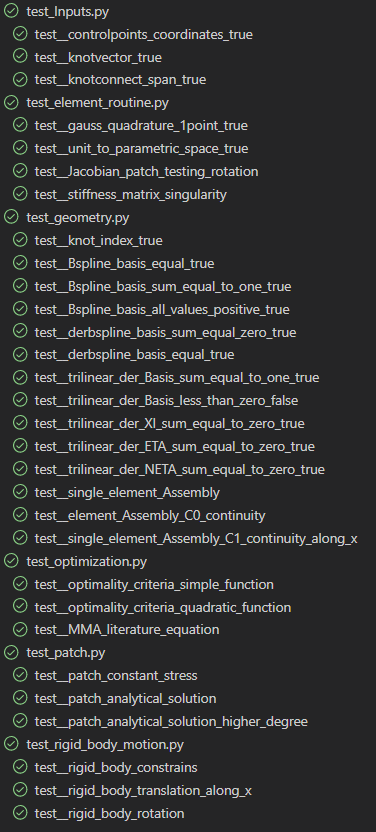
\includegraphics[width=0.25\linewidth]{list_of_tests.png}
\caption{List of test cases }
\label{fig:List of test cases}
\end{figure}
\begin{enumerate}
\item test$\_$Inputs.py $\colon$ Test cases for input parameters

\item test$\_$geometry.py $\colon$ Test cases on  shape function and assembly 

\item test$\_$element$\_$routine.py $\colon$ Test cases on integration scheme and sanity checks on other element.

\item test$\_$optimization.py $\colon$ Test cases on optimizer function OC(optimality criterion) and MMA(method of moving asymptotes)

\item test$\_$rigid$\_$body$\_$motion.py $\colon$ Test cases to validate global stiffness matrix and boundary conditions by performing rigid body translation and rotation.

\item test$\_$patch.py $\colon$ Test cases on constant stress patch test and comparing analytical solution with numerical for lower and higher order shape functions.
\end{enumerate}
To run all the test cases, copy all test files in same folder and enter \textbf{PYTEST} command on the terminal.\\
Test commands to run the respective files.
\begin{lstlisting}
pytest test_Inputs.py
pytest test_geometry.py
pytest test_element_routine.py
pytest test_optimization.py
pytest test_patch.py
pytest test_rigid_body_motion.py
\end{lstlisting}

\end{subsection}
\end{section}

\begin{section}{RESULTS VALIDATION}

The input parameters are Length 8cm, Height 5cm, Width 1cm, Young's modulus 150000 N/m, Poisson ratio 0.3, load 100 N, volume fraction 0.4(optimized volume V/original volume V0), penalization factor 3, minimum radius 1.5 are same for all test cases only the boundary conditions change.\\ 
Degree of the curve\\
p=1,q=1,r=1.
\begin{subsection}{Validation case-1}

\subsubsection{Problem description}
Topology optimization of cantilever beam which is subjected to load at the free end. As shown in figure -\ref{fig:problem-1}
\begin{figure}[H]
	\begin{center}
		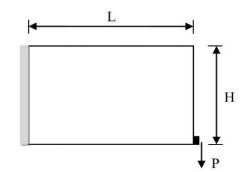
\includegraphics[scale=1]{Problem-1.png} 
		\caption{\\Cantilever beam with load at free end}\label{fig:problem-1}
	\end{center}	
\end{figure}
\subsubsection{Results}
\textit{see PPP document section 8.1}\\
1.\textbf{MMA optimizer}
\begin{lstlisting}
INPUTS:
l h w nx ny nz load volume_fra penal rmin E v density BC_op Ft_op verbose
8 5 1 35 25 3 -100 0.4 3 1.5 150000 0.35 7850 0 1 1
\end{lstlisting}

\begin{figure}[H]
	\centering
	\begin{minipage}{.5\textwidth}
		\centering
		
\includegraphics[width=0.5\linewidth]{analytical_1.png}
		\captionof{figure}{IGTO validation-1 for MMA
			\\\textbf{Results from literature}}
		\label{VC-01.1}
	\end{minipage}%
	\begin{minipage}{0.5\textwidth}
		\centering
		\includegraphics[width=0.5\linewidth]{Numerical_result_MMA_01.png}
		\captionof{figure}{Optimized structure using MMA method\\ 
		\textbf{Program generated result, plotted in paraview}}
		\label{VC-01.2}
	\end{minipage}
\end{figure}

2.\textbf{OC optimizer}
\begin{lstlisting}
INPUTS:
l h w nx ny nz load volume_fra penal rmin E v density BC_op Ft_op verbose
8 5 1 35 25 3 -100 0.4 3 1.5 150000 0.35 7850 0 0 1
\end{lstlisting}

\begin{figure}[H]
	\centering
	\begin{minipage}{.5\textwidth}
		\centering
		
\includegraphics[width=0.5\linewidth]{analytical_OC_1.png}
		\captionof{figure}{IGTO validation-1 for OC
			\\\textbf{Results from literature}}
		\label{VC-01.1}
	\end{minipage}%
	\begin{minipage}{0.5\textwidth}
		\centering
		\includegraphics[width=0.5\linewidth]{Numerical_result_OC_01.png}
		\captionof{figure}{Optimized structure using OC method\\ 
		\textbf{Program generated result, plotted in paraview}}
		\label{VC-01.2}
	\end{minipage}
\end{figure}

\end{subsection}
\begin{subsection}{Validation case-2}
\textit{see PPP document section 8.2}
\subsubsection{Problem description}
Topology optimization of cantilever beam which is subjected to load acting at the center of the free end. As shown in figure -\ref{fig:problem-2}
\begin{figure}[H]
	\begin{center}
		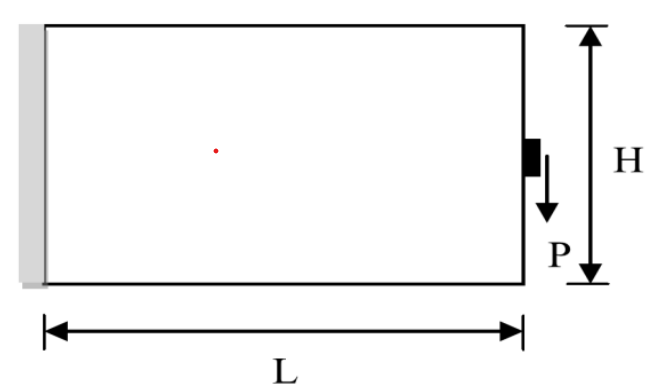
\includegraphics[scale=0.25]{Problem-2.png} 
		\caption{\\Cantilever beam with load at the center of the free end}\label{fig:problem-2}
	\end{center}	
\end{figure}
\subsubsection{Results}
1.\textbf{MMA optimizer}
\begin{lstlisting}
INPUTS:
l h w nx ny nz load volume_fra penal rmin E v density BC_op Ft_op verbose
8 5 1 35 25 3 -100 0.4 3 1.5 150000 0.35 7850 0 1 1
\end{lstlisting}

\begin{figure}[H]
	\centering
	\begin{minipage}{.5\textwidth}
		\centering
		
\includegraphics[width=0.5\linewidth]{analytical_OC_2.png}
		\captionof{figure}{IGTO validation-1 for MMA
			\\\textbf{Results from literature}}
		\label{VC-03.1}
	\end{minipage}%
	\begin{minipage}{0.5\textwidth}
		\centering
		\includegraphics[width=0.5\linewidth]{Numerical_result_MMA_02.png}
		\captionof{figure}{Optimized structure using MMA method\\ 
		\textbf{Program generated result, plotted in paraview}}
		\label{VC-03.2}
	\end{minipage}
\end{figure}
2. \textbf{OC optimizer}
\begin{lstlisting}
INPUTS:
l h w nx ny nz load volume_fra penal rmin E v density BC_op Ft_op verbose
8 5 1 35 25 3 -100 0.4 3 1.5 150000 0.35 7850 0 0 1
\end{lstlisting}

\begin{figure}[H]
	\centering
	\begin{minipage}{.5\textwidth}
		\centering
		
\includegraphics[width=0.5\linewidth]{analytical_OC_2.png}
		\captionof{figure}{IGTO validation-2 for OC
			\\\textbf{Results from literature}}
		\label{VC-01.1}
	\end{minipage}%
	\begin{minipage}{0.5\textwidth}
		\centering
		\includegraphics[width=0.5\linewidth]{Numerical_result_OC_02.png}
		\captionof{figure}{Optimized structure using OC method\\ 
		\textbf{Program generated result, plotted in paraview}}
		\label{VC-01.2}
	\end{minipage}
\end{figure}

\end{subsection}
\begin{subsection}{Validation case-3}
\subsubsection{Problem description}
Topology optimization of simple supported beam which is subjected to load acting at the center. As shown in figure -\ref{fig:problem-3}
\begin{figure}[H]
	\begin{center}
		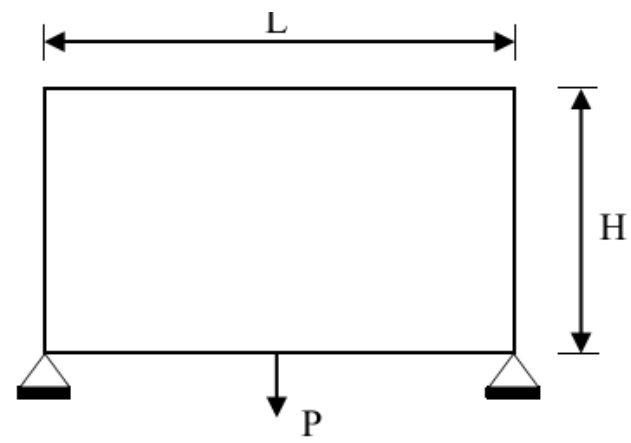
\includegraphics[scale=0.25]{Problem-3.png} 
		\caption{\\Simple supported beam with load at the center of the free end}\label{fig:problem-3}
	\end{center}	
\end{figure}
\subsubsection{Results}
\textit{see PPP document section 8.3}\\
1.\textbf{MMA optimizer}
\begin{lstlisting}
INPUTS:
l h w nx ny nz load volume_fra penal rmin E v density BC_op Ft_op verbose
8 5 1 35 25 3 -100 0.4 3 1.5 150000 0.35 7850 0 1 1
\end{lstlisting}

\begin{figure}[H]
	\centering
	\begin{minipage}{.5\textwidth}
		\centering
		
\includegraphics[width=0.5\linewidth]{analytical_3.png}
		\captionof{figure}{IGTO validation-3 for MMA
			\\\textbf{Results from literature}}
		\label{VC-03.1}
	\end{minipage}%
	\begin{minipage}{0.5\textwidth}
		\centering
		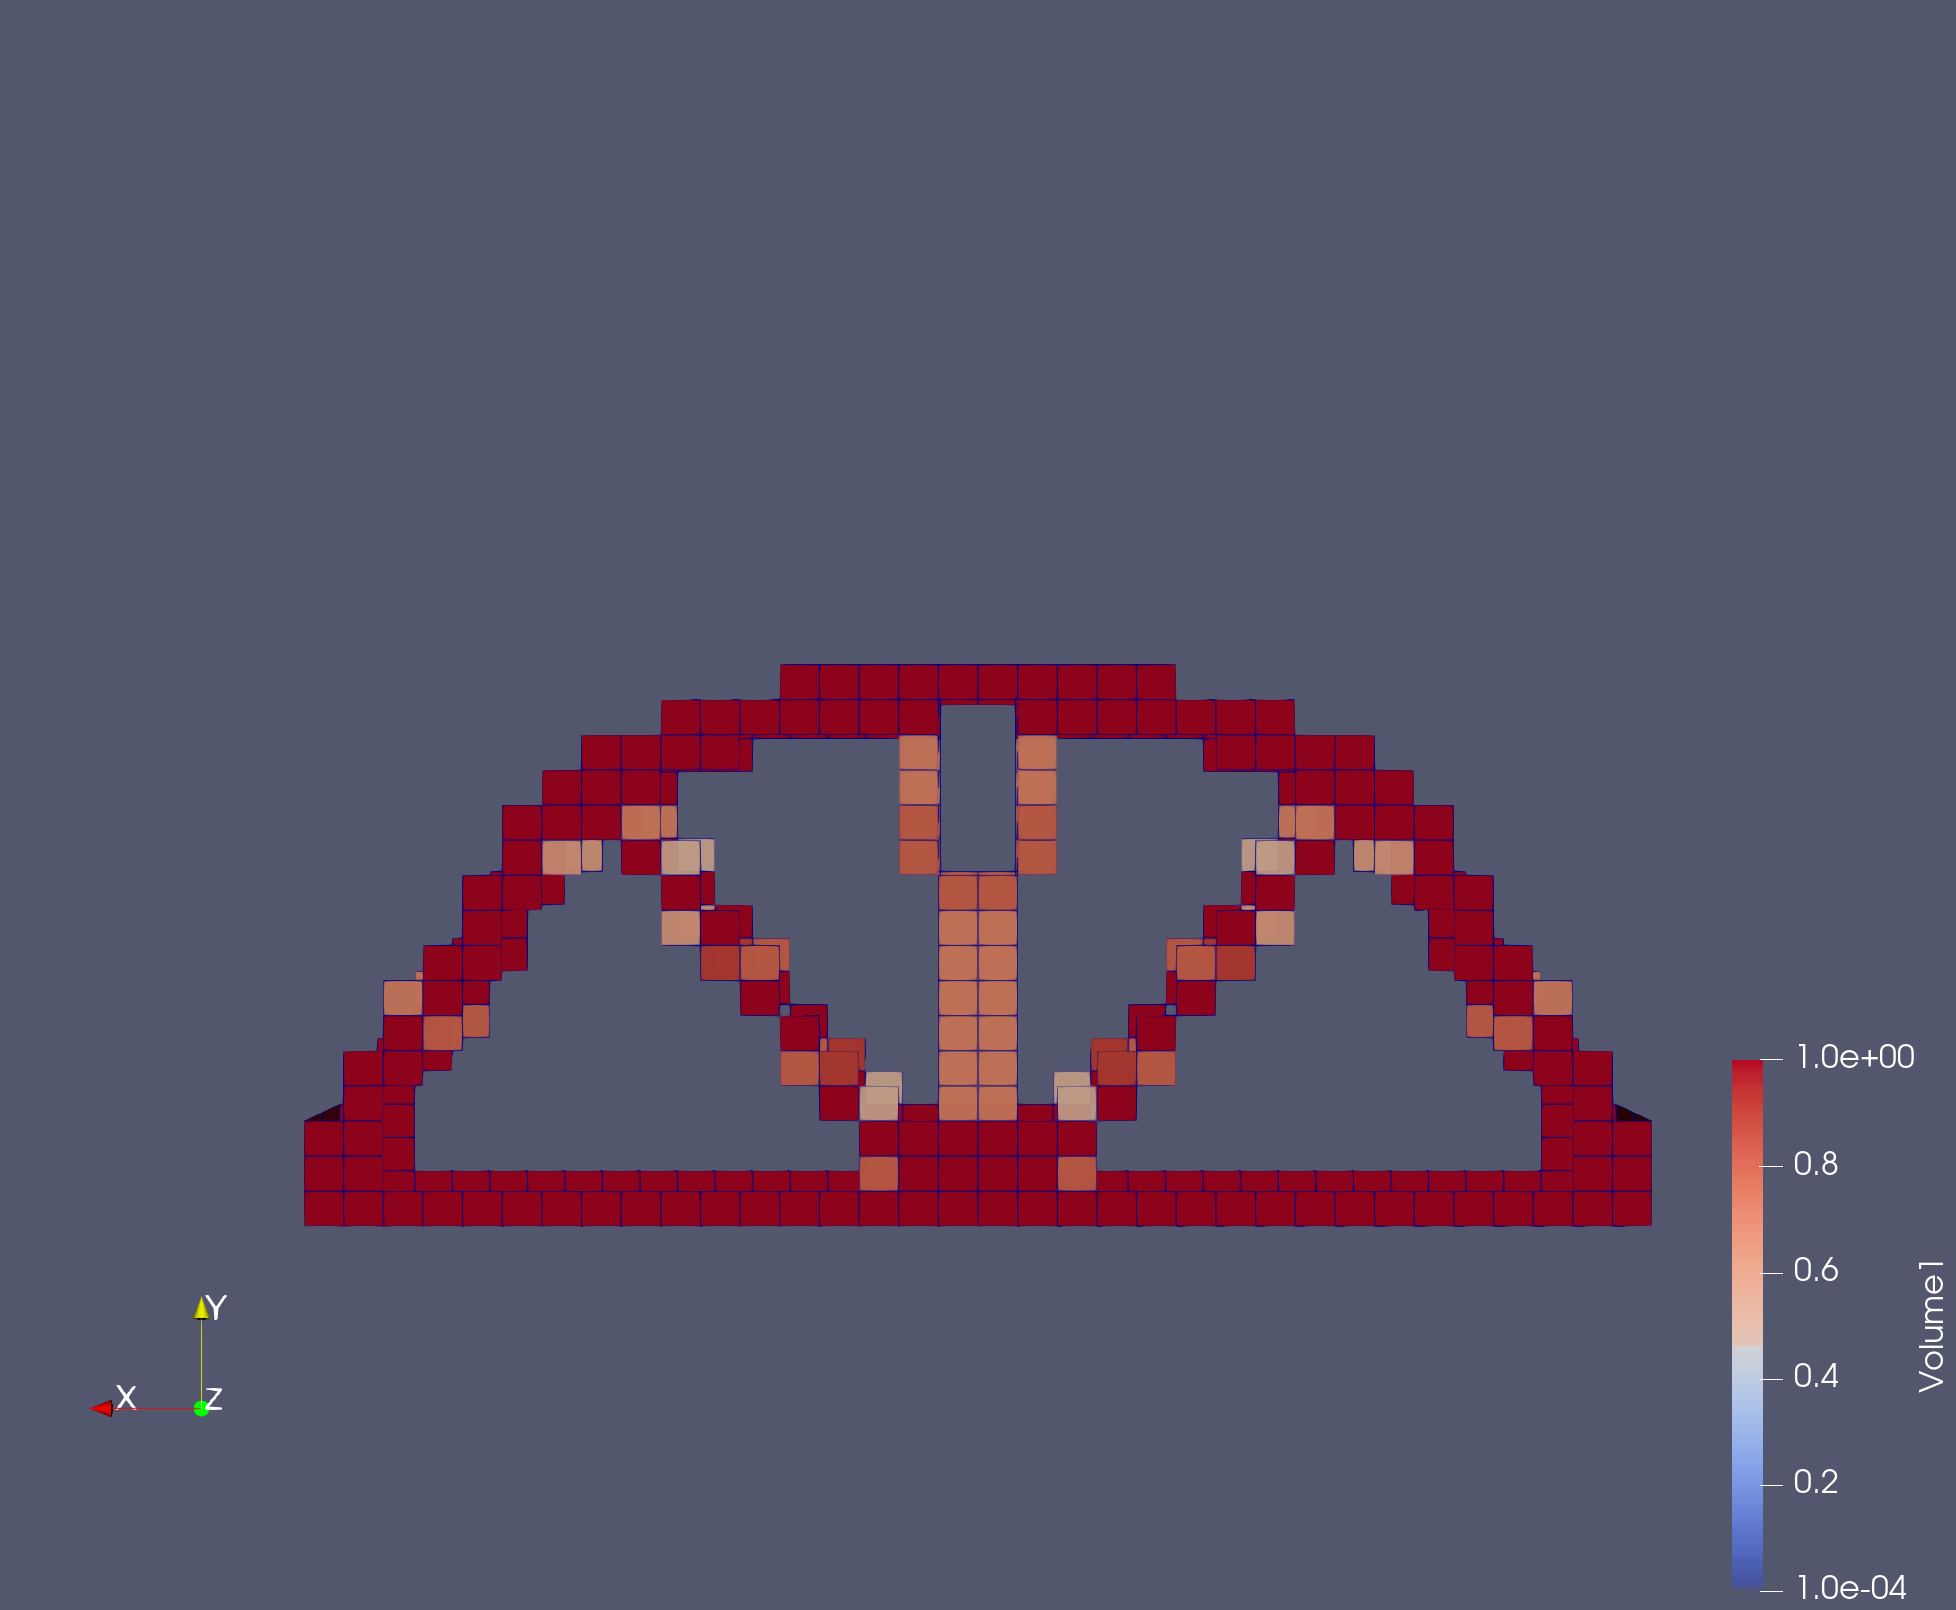
\includegraphics[width=0.5\linewidth]{Numerical_result_MMA_03.png}
		\captionof{figure}{Optimized structure using MMA method\\ 
		\textbf{Program generated result, plotted in paraview}}
		\label{VC-03.2}
	\end{minipage}
\end{figure}

2. \textbf{OC optimizer}
\begin{lstlisting}
INPUTS:
l h w nx ny nz load volume_fra penal rmin E v density BC_op Ft_op verbose
8 5 1 35 25 3 -100 0.4 3 1.5 150000 0.35 7850 0 0 1
\end{lstlisting}

\begin{figure}[H]
	\centering
	\begin{minipage}{.5\textwidth}
		\centering
		
\includegraphics[width=0.5\linewidth]{analytical_3.png}
		\captionof{figure}{IGTO validation-2 for OC
			\\\textbf{Results from literature}}
		\label{VC-01.1}
	\end{minipage}%
	\begin{minipage}{0.5\textwidth}
		\centering
		\includegraphics[width=0.5\linewidth]{Numerical_result_OC_03.png}
		\captionof{figure}{Optimized structure using OC method\\ 
		\textbf{Program generated result, plotted in paraview}}
		\label{VC-01.2}
	\end{minipage}
\end{figure}

\end{subsection}
\newpage
NOTE:
\begin{enumerate}
\item Recommended to use SYPDER (ANACONDA) python IDE for better visualization of output if using PYVISTA.
\item if the program is not able to plot results, enter verbose as 0.
\begin{lstlisting}
INPUTS:
l h w nx ny nz load volume_fra penal rmin E v density BC_op Ft_op verbose
8 5 1 35 25 3 -100 0.4 3 1.5 150000 0.35 7850 0 0 0
\end{lstlisting}
\item visualization of optimized structure can be done using the VTK file generated in paraview. For more details see \textit{PPP document section 5.5.2}
\end{enumerate}
\end{section}
\end{document}